\documentclass{projekt}
\usepackage[none]{hyphenat}
\usepackage{url}
\usepackage[utf8]{inputenc}
\usepackage[T1]{fontenc} 
\usepackage{ae}
\usepackage{fancyhdr}
\usepackage{graphicx}
\usepackage{pdfpages}
\usepackage[all]{xy}
\usepackage[czech]{babel}
\usepackage[activate={true,nocompatibility,all}, stretch=10, shrink=10, step=1, auto=true, draft=false]{microtype}
%\usepackage[total={17cm,28cm}, top=3cm, left=2cm, includefoot]{geometry}
\frenchspacing
\author{Filip Markvart}
\title{Datový model EEG/ERP portálu v prostředcích sémantického webu}
\titlet{} 
\titlett{}
\university{Západočeská univerzita v Plzni}
\faculty{Fakulta aplikovaných věd}
\department{Katedra informatiky a výpočetní techniky}
\subject{Diplomová práce}
\town{Plzeň}
\begin{document}
\pagestyle{fancy}
\renewcommand{\chaptermark}[1]{\markboth{\textit{#1}}{}}
\renewcommand{\sectionmark}[1]{\markright{\textit{#1}}{}}
\cfoot{\thepage}
\lhead{\leftmark}
\rhead{\rightmark}
\maketitle
\chapter*{Prohlášení}
\thispagestyle{empty}
Prohlašuji, že jsem diplomovou práci vypracoval samostatně a výhradně s~použitím citovaných pramenů.
\vskip 1.5em
V Plzni dne \today
\vskip 0.7em
\hskip 9cm Filip Markvart
\chapter*{Abstract}
\thispagestyle{empty}
\hspace{0.65cm}This thesis DODELAT
%describes a transformation of neuroinformatics metadata stored in the relational database to the semantic web standard. The main goal is to investigate existing tools and necessary %modifications that ensure automatic transformation for converting input data. The modified tool is able to process additional semantic information that cannot be stored in the relational %database.


%The last part describes design and implementation of an application that uses annotations to add semantic information to transformed data.

\tableofcontents
\pagestyle{fancy}
\renewcommand{\chaptermark}[1]{\markboth{\textit{#1}}{}}
\renewcommand{\sectionmark}[1]{\markright{\textit{#1}}{}}
\cfoot{\thepage}
\lhead{\leftmark}
\rhead{\rightmark}
\parskip 1em
\chapter{Úvod}
\hspace{0.65cm}EEG/ERP portál je webová aplikace sloužící výzkumným pracovníkům ke shromažďování a organizaci dat získaných při neuroinformatických experimen-\\tech v EEG laboratoři. Jejím cílem je ukládání naměřených dat v kontextu prováděného experimentu, který lze popsat rozsáhlou množinou různorodých údajů. Tato aplikace již prošla mnohaletým vývojem v jehož průběhu postupně docházelo ke změnám datového modelu kvůli přibývajícím požadavkům na uchovávaná data. Relační databáze jež slouží jako persistentní úložiště tak postupně byla rozšiřována o další tabulky, jejichž počet se k datu tvorby této práce pohybuje v řádu desítek. Většina realizací požadavků na ukládání dalších dat tak přímo znamená zásah nejen do databáze portálu ale také to do datové vrstvy, která ji využívá. V současné době tak databáze obsahuje velké množství tabulek uchovávající různá data, která jsou ale ve smyslu sémantiky často příbuzná a existuje mezi nimi vazba, která je prostřednictvím relačního datového modelu velmi obtížně popsatelná. Zároveň lze očekávat, že budou přibývat požadavky na uchování dalších dat, která navíc nemusejí mít jen homogenní strukturu (ve smyslu relační databáze), ale může se jednat i o množiny sémanticky příbuzných údajů – tzv. metadata, které budou vázány pouze k některým datům. Možnost ukládání strukturně heterogenních, ale sémantický příbuzných metadat je tak dalším otevřeným problémem.

Cílem této práce je prozkoumání struktury a nalezení sémantiky dat v současném datovém modelu relační databáze portálu a následná úprava tohoto modelu do podoby, která by dovolovala uchovat jak sémantiku dat, kterou není možné relačním modelem vyjádřit tak dodávat dynamicky datům přídavná metadata, aniž by muselo docházet k větším zásahům do datového modelu portálu. Pro realizaci úpravy datového modelu budou v této práci využity prostředky tzv. sémantického webu, který poskytuje množství standar-\\dů a technologií pro uchovávání organizaci a správu dat. Tyto technologie a nástroje zde budou popsány a na základě jejich analýzy budou vybrány prostředky, které se využijí pro implementaci úpravy zmiňovaného datového modelu. 
Poslední část práce se věnuje testování modifikovaného modelu a to především z výkonnostního hlediska. Díky této části by mělo být možné posoudit jak užitečnost samotné úpravy tak i použitelnost a efektivnost získaného modelu pro potřeby EEG/ERP portálu.


\chapter{Sémantický web}
\hspace{0.65cm}Dnešní podoba webu, tak jak je všeobecně známa, je tvořena značným množstvím informací, které mají řadu autorů, v podobě různých organizací či jednotlivců, jež se liší jak svým obsahem tak i podobou publikace. Tyto informace jsou poměrně snadno přístupné díky jejich jednoznačné identifikaci prostřednictvím URI identifikátoru (za předpokladu, že jej známe). K usnadně-\\ní získávání dalších (často příbuzných) informací napomáhají tzv. hypertexto-\\vé odkazy, jež usnadňují přístup k dalším zdrojům informací odstraněním požadavku na uživatelovu znalost identifikátoru cílového zdroje. Samotné hypertextové odkazy tak sice zajišťují provázání jednoho informačního zdroje s jiným díky znalosti jeho URI identifikátoru, ale nenesou už žádné další informace, které by například uživateli poskytly další údaje o cílovém zdroji. 
Takováto podoba umožňuje získávání informací jak koncovým uživatelům webu, tak v omezené podobě i vyhledávacím strojům, ale má své limity, neboť se v nepřeberném množství dat lze snadno ztratit, či se jen dostat k irelevantním informacím \cite{_1}.
Základním úkolem sémantického webu, jehož první myšlenky prezentoval v roce 2001 zakladatel konsorcia W3C Tim Berners-Lee, je umožnit aby informace dostupné prostřednictvím webu byly srozumitelné nejen uživatelům, ale také počítačům, jež tato data zpracovávají \cite{_2}. Hlavním cílem je tedy vývoj standardů a technologií, které by umožňovaly přesnější a podrobnější vyhledávání, integraci dat a také automatizaci častých úkonů. 
Sémantický web je založen na několika principech, které budou níže uvedeny.

\begin {itemize}

\item \textbf{Jednoznačná identifikace entit prostřednictvím URI}

\hspace{0.65cm}Veškerá data, reprezentující obvykle objekty reálného světa publikovaná prostřednictvím webu je možné jednoznačně odkazovat prostřednictvím identifikátoru URI. Díky této skutečnosti je tak možné realizovat i nepřímé odkazy na objekty, například osobu Petr Novák s emailem petr.novak@w3.org je možné identifikovat jako osobou, jejíž email má URI mailto:petr.novak@w3.org.


\item \textbf{Zdroje i odkazy mezi nimi je možné typovat}

\hspace{0.65cm}Současná podoba webu je tvořena zdroji a odkazy jež je vzájemně propojují. Zdroje, které jsou reprezentovány webovými dokumenty jsou publikovány za účelem poskytnutí informací lidskému uživateli, který dokáže ze samotného obsahu dokumentu získat i některá jeho metadata (pokud jsou v určité formě součástí obsahu) a do jisté míry také vztah k ostatním dokumentům, na něž vedou případné odkazy. Stroje v podobě různých vyhledávačů či automatů pro shromažďování dat ale tuto schopnost nemají nebo je pro ně příliš náročná. Řešením sémantického webu je typování jak samotných zdrojů, tak i odkazů, které je provazují. Díky této skutečnosti je pak možné webovým dokumentům dodávat metadata jako např. autora, verzi či závislost na jiném dokumentu. Z hlediska typování odkazů je například možné jeden webový zdroj označit pouze jako odlišnou verzi jiného zdroje.


\item \textbf{Tolerance neúplných informací}

\hspace{0.65cm}U současně podoby webu může nastat situace, kdy některý zdroj není dostupný. V takovém případě uživatel ztrácí přistup k danému dokumentu, ale díky koncepci webu není nikterak ohrožena dostupnost ostatních zdrojů. V případě sémantického webu se situace nemění, nedostupnost některého zdroje není žádnou překážkou, neboť nástroje sémantického webu zpracovávají pouze ty informace, které jsou dostupné a těch vytvářejí závěry. V důsledku je tak možné dojít při zpracovávání dat ke stejným výsledkům, jako v případě, když jsou zpracovávány jen některé vybrané informace, jejichž rozsah je explicitně definován.

\item \textbf{Zpracování neověřených dat}

\hspace{0.65cm}Při zpracování informací pocházejících z neověřených zdrojů je možné dohledávat prostřednictvím typovaných odkazů důvěryhodná data, jejichž obsah a odkazy poslouží jako ověřovací prostředek. Tento princip je možné uvést na jednoduchém příkladu. Aplikace zpracovávající data sémantického webu vyhledá informace, přičemž je kladen požadavek na vysokou pravděpodobnost správnosti výsledku. Pokud část nalezených informací pochází z neověřeného zdroje, je možné vyhledávat například jejich autora v odkazech zdrojů, které jsou důvěryhodné. V případě úspěchu nalezení takového odkazu u více různých zdrojů je pak možné považovat zkoumaný zdroj s vysokou pravděpodobností rovněž za důvěry-\\hodný a tím zajistit plnění požadavků na výsledek.

\item \textbf{paralelního vývoje dat}

\hspace{0.65cm}V průběhu času nezřídka nastávají situace, kdy autoři, či skupiny autorů publikují obdobná data na různých místech nebo v odlišném čase. Obsah těchto dokumentů se může navíc lišit svým jazykem či použitou terminologií, ač význam bude shodný. S využitím prostředků sémantického webu je ale možné prostřednictvím typovaných odkazů zajistit provázanost významově obdobných či na sebe navazujících dat i přes překážku rozdílnosti jejich podoby zápisu. Navíc je také možné dodávat nové informace bez nutnosti úpravy původních dat, která tím pádem nezmění svoji strukturu \cite{_1}.

\end{itemize}


\section{Architektura sémantického webu}
\hspace{0.65cm}Architektura sémantického webu sestává z více oddělených vrstev, mezi nimiž je zajištěna zpětná i dopředná kompatibilita \cite{_3}. Nejnižší vrstva je tvořena dvěma technologickými standardy – URI identifikátory sloužící pro jednoznačné pojmenování zdrojů dat a Unicode kódování mezinárodní znako-\\vou sadou. Druhou vrstvu architektury, jež je patrná z obrázku 2.1, reprezentu-\\je značkovací jazyk XML (Extensible Markup Language), který umožňuje tvorbu strukturovaného dokumentu za užití vlastních značek. Tato vrstva zároveň zajišťuje definici XML schématu včetně jmenných prostorů. RDF + rdfschema jež následuje je klíčovou vrstvou sémantického webu neboť dovoluje tvorbu vazeb a vztahů mezi jednotlivými zdroji, které jsou typované spolu s odkazy. Je tak možné definovat libovolné vztahy mezi objekty či jejich kategoriemi bez nutnosti specifikace významu samotných vazeb či objektů. Díky RDF schématu je vytvářena základní sémantika datového modelu, která už definuje význam některých elementů jako třídy či podtřídy. 
Vrstva ontologického slovníku, zastoupená jazykem OWL, nabízí pokročilou reprezentaci znalostí na úrovni deskripční logiky a umožňuje tak vytvářet složitější struktury sloužící k popisu různých vlastností objektů \cite{_2}. Poslední vrstvou, která je jako všechny předchozí zmíněné konsorciem W3C standardizo-\\vaná jsou digitální podpisy. Ty poskytují možnosti například pro detekci různých verzí dokumentů. Zbylé výše znázorněné vrstvy slouží pro definice a vyhodnocování odvozovacích pravidel a v současnosti jsou ve fázi vývoje \cite{_1}.

\begin{figure}[htb]
\begin{center}
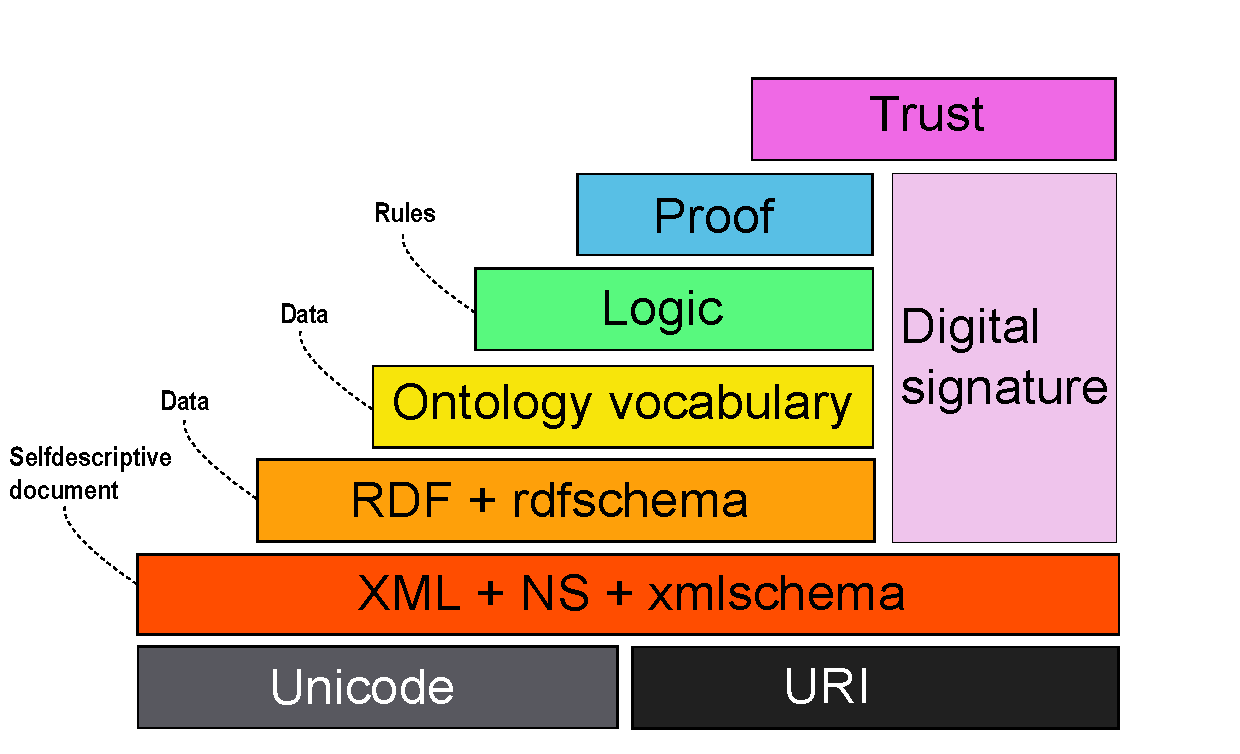
\includegraphics[scale=0.62]{architektura.pdf}
\caption{Architektura sémantickém webu \cite{_1}}
\end{center}
\end{figure}

Vrstvení jazyků sémantického webu je podstatné pro úroveň expresivity znalostního modelu, neboť s rostoucí vyjadřovací možností jazyka také roste složitost dotazovacích operací nad modelem. Je tedy nutné před započetím tvorby modelu nejprve zjistit jeho požadovanou expresivitu a podle té zvolit pro zápis dat jazyk, který ji dovoluje obsáhnout. Využívá se tedy skutečnosti, že jazyk vyšší vrstvy zahrnuje vyjadřovací schopnosti vrstev nižších\cite{_2}. 
Další podkapitoly se budou zabývat podrobněji jednotlivý zmíněnými technologiemi.

\section{XML}
\hspace{0.65cm}XML (eXtensible Markup Language) je značkovací jazyk sloužící pro popis hierarchických struktur textových dokumentů prostřednictvím tzv. tagů. Tag je konstrukce, která slouží k počátečnímu a koncovému ohraničení společně definovaného elementu. Tag lze chápat jako prostředek pro dodání metadat ke textové struktuře, jež ohraničuje. Příkladem může být následující zápis {\it <prijmeni>Novák</prijmeni>}, kde elementu {\it Novák} je dodána meta informace, že se jedná o příjmení. Samotné XML ale nedefinuje žádný sémantický význam tagů, slouží pouze pro specifikaci syntaxe na úrovní XML dokumentu. Pro definici (zejména hierarchické) struktury XML dokumentu slouží XML Schema, které umožňuje zápis pravidel, jež musí cílový dokument dodržovat pro zachování své validity. Ze strany sémantického webu ale nemají pravidla XML Schema žádný sémantický význam a slouží tak pouze pro definici struktury a syntaxe. Zmíněné schéma také definuje základní datové typy (čísla, řetězce, čas a pod.), které nabývají významu v sémantických jazycích jako je RDF \cite{_3}.


\section{RDF}
\hspace{0.65cm}Technologický základ sémantického webu tvoří jazyk RDF (Resource Description Framework), jež slouží jako obecný rámec pro popis, výměnu a opětovné použití metadat \cite{_3}. Tento rámec poskytuje jednoduchý model sloužící pro popis zdrojů jež je nezávislý na jeho konkrétní implementaci \cite{_4}. Samotné informace o objektu jsou realizovány prostřednictvím tvrzení, jež se označují jako trojice (anglicky triple). Každou trojici tvoří spolu subjekt, predikát a objekt. Subjekt je libovolný objekt identifikovatelný pomocí URI, který se snažíme prostřednictvím trojice popisovat, zaznamenat nějakou jeho vlastnost. Tato vlastnost se popisuje prostřednictvím predikátu, který vede ve směru od subjektu ke objektu, přiřazuje tedy subjektu nějaký objekt prostřednictvím této vlastnosti. Cílový objekt pak představuje hodnotu, které předchozí objekt nabývá pro daný predikát. 
Tento princip je možné znázornit na jednoduchém tvrzení, zapsaném větou „Martin staví dům.“ Subjektem trojice potom bude Martin, predikátem staví a objektem dům, tak jak je znázorněno na obrázku 2.2. 
\\
\vspace{0.1cm}

\begin{figure}[htb]
\begin{center}
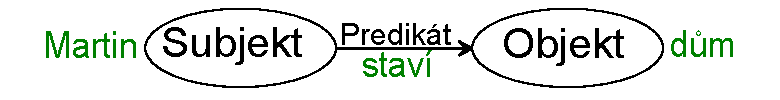
\includegraphics[scale=0.9]{trojice.pdf}
\caption{Příklad RDF trojice}
\end{center}
\end{figure}

Dle definovaného standardu \cite{_5} je možné, aby objektem byl jiný subjekt. Díky této skutečnosti je možné jednotlivé trojice spojovat do většího celku, který ve výsledku tvoří strukturu orientovaného grafu, kterou lze označit jako model \cite{_3}. Jednoduchým model tvořený dvěma trojicemi lze vytvořit využitím dalšího tvrzení „Dům stojí v Plzni.“ V předchozí trojici pak bude dům subjektem namísto objektu a dojde tak ke spojení dvou trojic (za předpokladu že v obou tvrzeních je myšlen stejný fyzický dům), tak jak je znázorněno na obrázku 2.3. 

\begin{figure}[htb]
\begin{center}
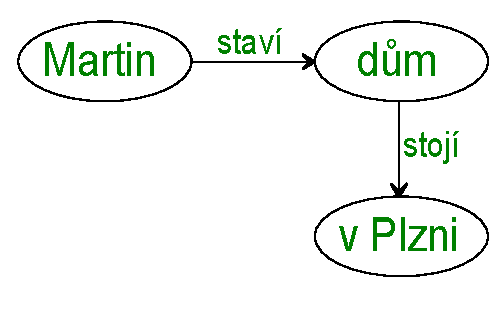
\includegraphics[scale=0.9]{miniStrom.pdf}
\caption{Příklad jednoduchého RDF modelu}
\end{center}
\end{figure}


Z hlediska implementace mohou být uzly orientovaného grafu datového modelu tvořeny URI identifikátorem, anonymním listem nebo literálem \cite{_6}. URI identifikátor obsahuje pouze adresu zdroje v textové podobě ve znakové sadě Unicode a zastupuje tak konkrétní jedinečný objekt. Anonymní list (anglicky blank node) je prvek nahrazující URI identifikátor při absenci unikátní adresy zdroje. Tato entita přestavuje zdroj, který je sice v rámci grafu popisován prostřednictvím trojic, ale není potřeba (často z hlediska významu), aby byl dostupný i vně grafu. S URI má společné to, že musí nést adresu zdroje (její syntaxe není implicitně definována), ale liší se skutečností, že tato adresa musí být unikátní pouze v rámci obalujícího modelu, nikoliv vně grafu. Může tak nastat situace, že dva odlišné modely budou obsahovat (ze syntaktického hlediska) dva stejné anonymní uzly, což v případě URI možné není (při respektování specifikace). Tento list tak může představovat anonymní objekt sloužící ke vytvoření vazby mezi jinými objekty, které jsou z hlediska sémantiky významné \cite{_5}. Jako příklad je možno uvést následující tvrzení. „Martinův přítel zná předpověď počasí. Počasí bude deštivé.„ Zjednodušeným převodem předchozích vět na trojice v podobě subjekt – predikát – objekt získáme: Martin – má – přítel, přítel – zná – počasí, počasí – bude – deštivé. 
Subjekt resp. objekt přítel zde může být reprezentován anonymním listem, v případě že jedinou signifikantní informací (z vnějšího pohledu na datový model) je Martinova získaná znalost počasí, nikoliv už jeho přítel, jež mu ji zprostředkoval. 
Poslední možnou reprezentací entity trojice je literál, jež nese Unicode textový řetězec, který slouží pro zápis koncové informace (užitečné pro lidského čtenáře). Literál může také navíc obsahovat položku, pro označení jazyka, ve kterém je textová informace zapsána \cite{_6}. 
\\
\\
Pro komponenty každé trojice grafu platí následující pravidla \cite{_6}.

\begin {itemize}

\item \textbf{subjekt} - může být tvořen URI identifikátorem nebo anonymním listem
\item \textbf{predikát} - může být tvořen pouze URI identifikátorem
\item \textbf{objekt} - může být tvořen URI, anonymním listem nebo literálem

\end{itemize}


Pro zápis trojic RDF grafu je sice možné využít grafické podoby, ale pro vyjádření sémantiky webových zdrojů je nejvhodnější využít syntaxe jazyka XML. Níže uvedená ukázka kódu reprezentuje XML zápis trojice z obrázku 2.2.

\begin{verbatim}
<rdf:RDF xmlns:rdf="http://www.w3.org/1999/02/22-rdf-syntax-ns#"
         xmlns:dc="http://purl.org/dc/elements/1.1/">
  <rdf:Description rdf:about="http://www.w3.org/Person/Martin">
    <dc:stavi>dům</dc:stavi>
  </rdf:Description>
</rdf:RDF>

\end{verbatim}

Samotné RDF nedefinuje trojicím ani jejím částem sémantiku, ale dovoluje vyjádřit základní vztahy náležitosti prvků do kategorie prostřednictvím kontejnerů a kolekcí (např. rdf:Bag, rdf:List) \cite{_2}. Pro dodání základní sémantiky slouží schéma popsané v následující podkapitole.

\section{RDFS}


\bibliography{diplomka}
\bibliographystyle{plain}


\end{document}
